\documentclass[a4paper,11pt]{article}
\usepackage[utf8]{inputenc}
\usepackage[T1]{fontenc}
\usepackage[french]{babel}
\usepackage[normalem]{ulem}
\usepackage{geometry}
\usepackage{lmodern}
\usepackage{graphicx}
\usepackage{setspace}
\usepackage{titlesec}
\usepackage{geometry}
\geometry{top=3cm, bottom=3cm, left=2cm, right=2cm}
\usepackage{placeins}
\usepackage{epsfig}
\usepackage{hyperref}
\usepackage{url}
\usepackage{cite}
\usepackage{listings}
\usepackage{xcolor}


%\lstset{
%language=Java,
%basicstyle=\normalsize, 
%upquote=true,
%aboveskip={1.5\baselineskip},
%columns=fullflexible,
%showstringspaces=false,
%extendedchars=true,
%breaklines=true,
%showtabs=false,
%showspaces=false,
%showstringspaces=false,
%identifierstyle=\ttfamily,
%keywordstyle=\color[rgb]{0,0,1},
%commentstyle=\color[rgb]{0.133,0.545,0.133},
%stringstyle=\color[rgb]{0.627,0.126,0.941},
%}

\title{Rapport\\Architecture Logicielle\\Jeu 2D autour d'un framework\\Année 2015/2016 }
\author{Raphaël Jorel, Antoine Laulan}



\begin{document}


\begin{figure}
    \begin{center}
    
\includegraphics[scale=0.7]{images/logo-bdx.pdf}
    \end{center}
\end{figure}
\maketitle

\newpage
\tableofcontents
\newpage



\newpage
\section{Introduction }
Notre jeu a été produit dans le cadre de l'UE architecture logicielle. Le but étant de créer un jeu à l'aide d'un framework fourni et cela sans modifier celui-ci.
Dans ce rapport nous présenterons notre jeu et nous fournirons une critique du framework utilisé.
%A voir si on laisse une intro, mais je trouve bizarre de pas en mettre en fait 

\section{Firewall Breaker}
\subsection{Présentation}
\FloatBarrier
		\begin{figure}[!h]
    		\begin{center}
	   	  	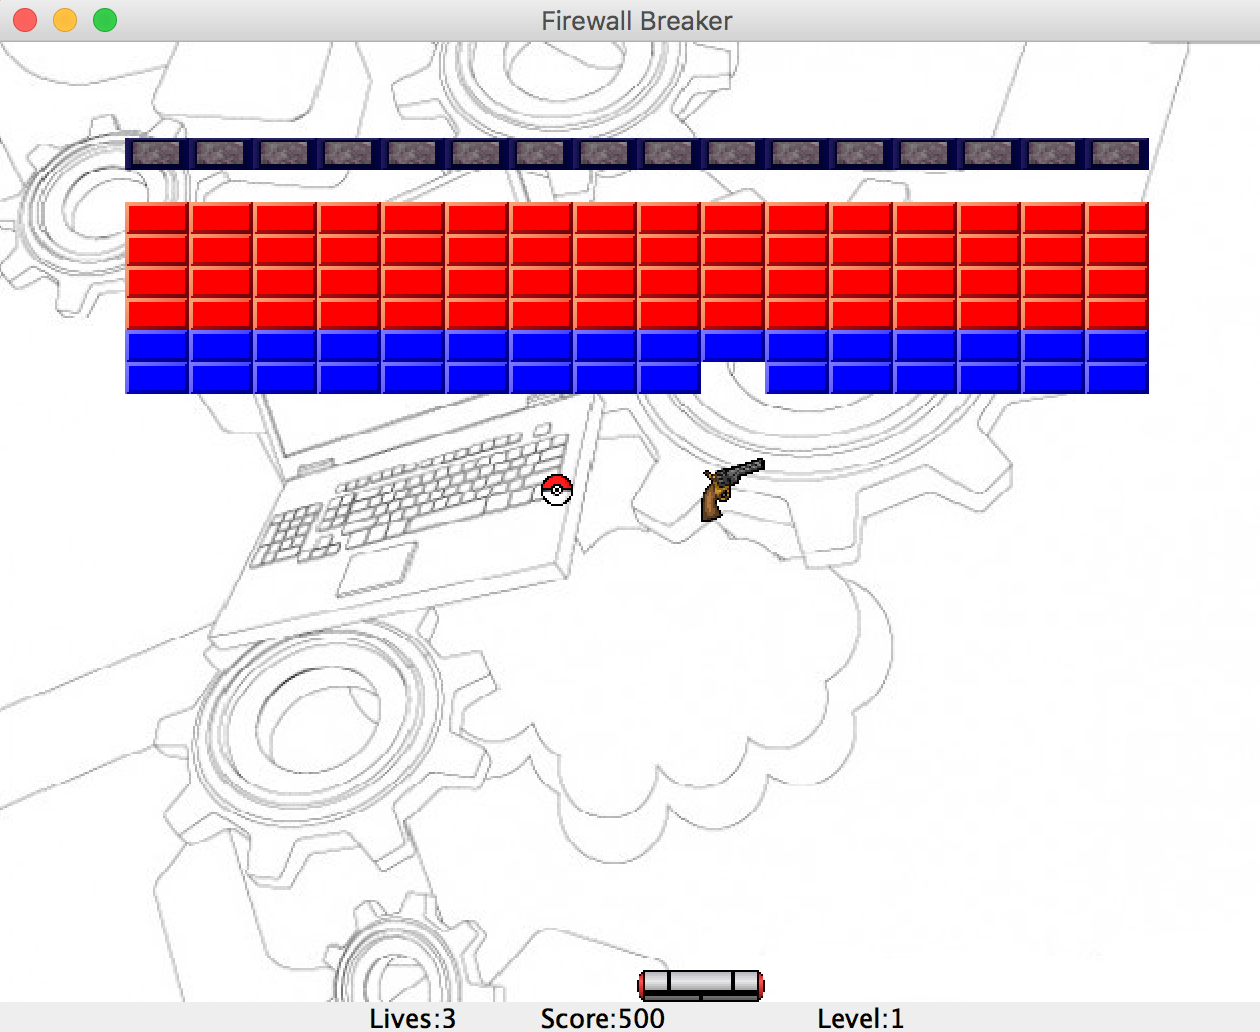
\includegraphics[scale= 0.5]{images/gameView.png}
          	\caption{Vue du jeu}
    		\end{center}
		\end{figure}
\FloatBarrier
Notre jeu est basé sur le principe d'un wall breaker. Le joueur contrôle une palette et doit, en faisant rebondir la balle, détruire les briques pour gagner.
Pour se faire il peut être aidé de divers bonus et briques spéciales. La partie s'arrête lorsque le joueur a détruit toutes les briques qui peuvent l'être, ou lorsque celui-ci n'a plus de vie.

\subsection{Fonctionnalités du jeu}
\begin{itemize}
\item 
\item
\item
\end{itemize}

\subsection{Architecture}
	Nous allons dans cette partie vous présenter l'architecture logicielle de notre jeu. Ceci sera fait à l'aide de diagrammes de classes.
	Nous metrons en évidence les connexions entre nos classes et les classes du framework.

% A voir si on met un diag de paquetage ou pas

	\subsubsection{Diagrammes de classe}
		
		\FloatBarrier
		\begin{figure}[!h]
    		\begin{center}
	  	  	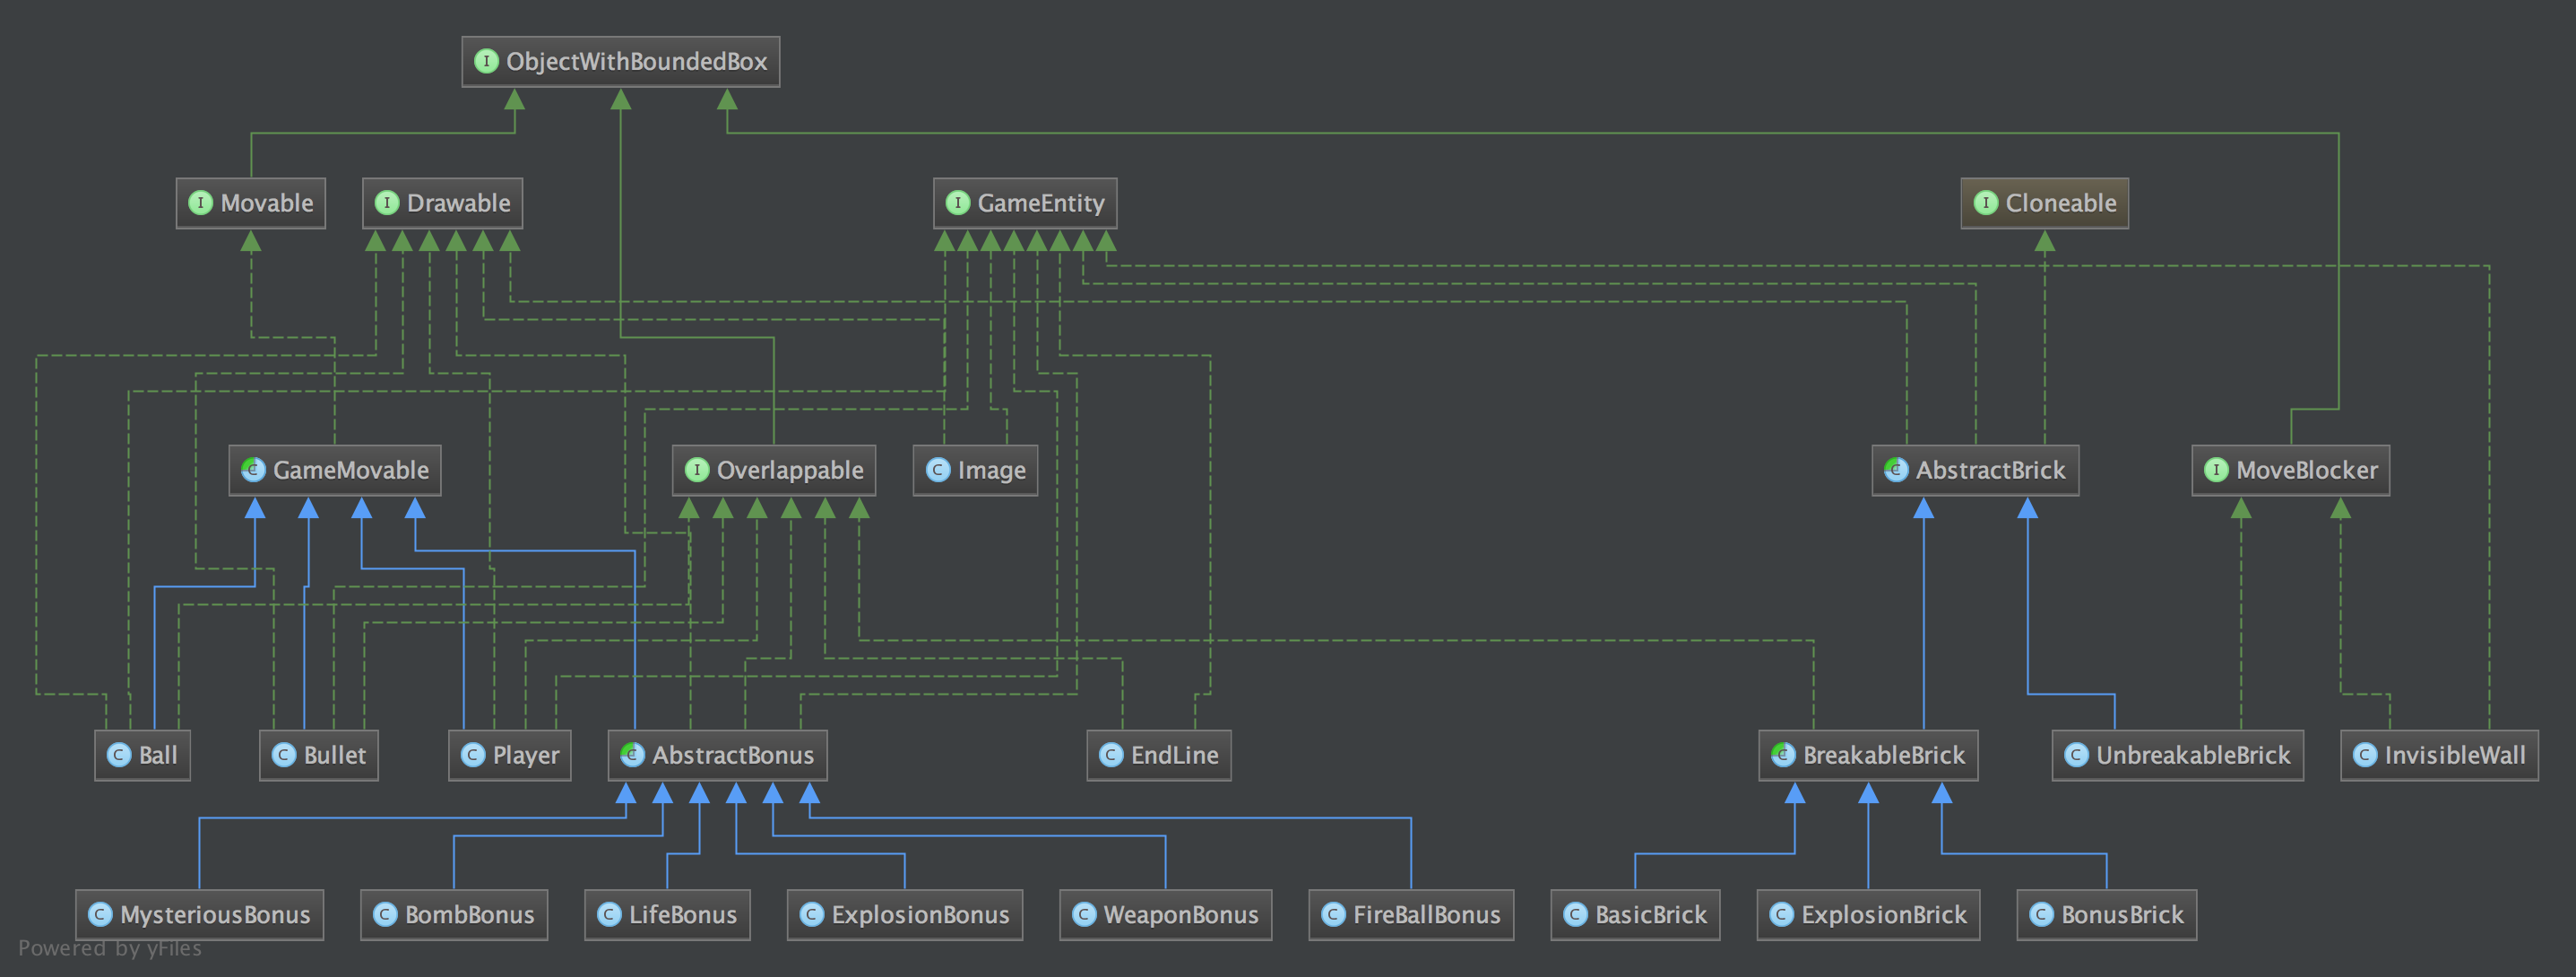
\includegraphics[scale=0.175]{images/entitiesDiag.png}
          	\caption{Diagramme de classe des entités}
    		\end{center}
		\end{figure}
		\FloatBarrier
		\paragraph{Description :}
		Voici le diagramme de classe regroupant les différentes entités de note jeu. \\
		
		% pour l'instant c'est dégeu mais c'est temporaire c'est juste histoire de poser le concept de couleur 
		% car plusieurs classes sont relations donc j'ai regroupé tout dans un diag que on va différencier par les couleurs
		\FloatBarrier
		\begin{figure}[!h]
    		\begin{center}
	  	  	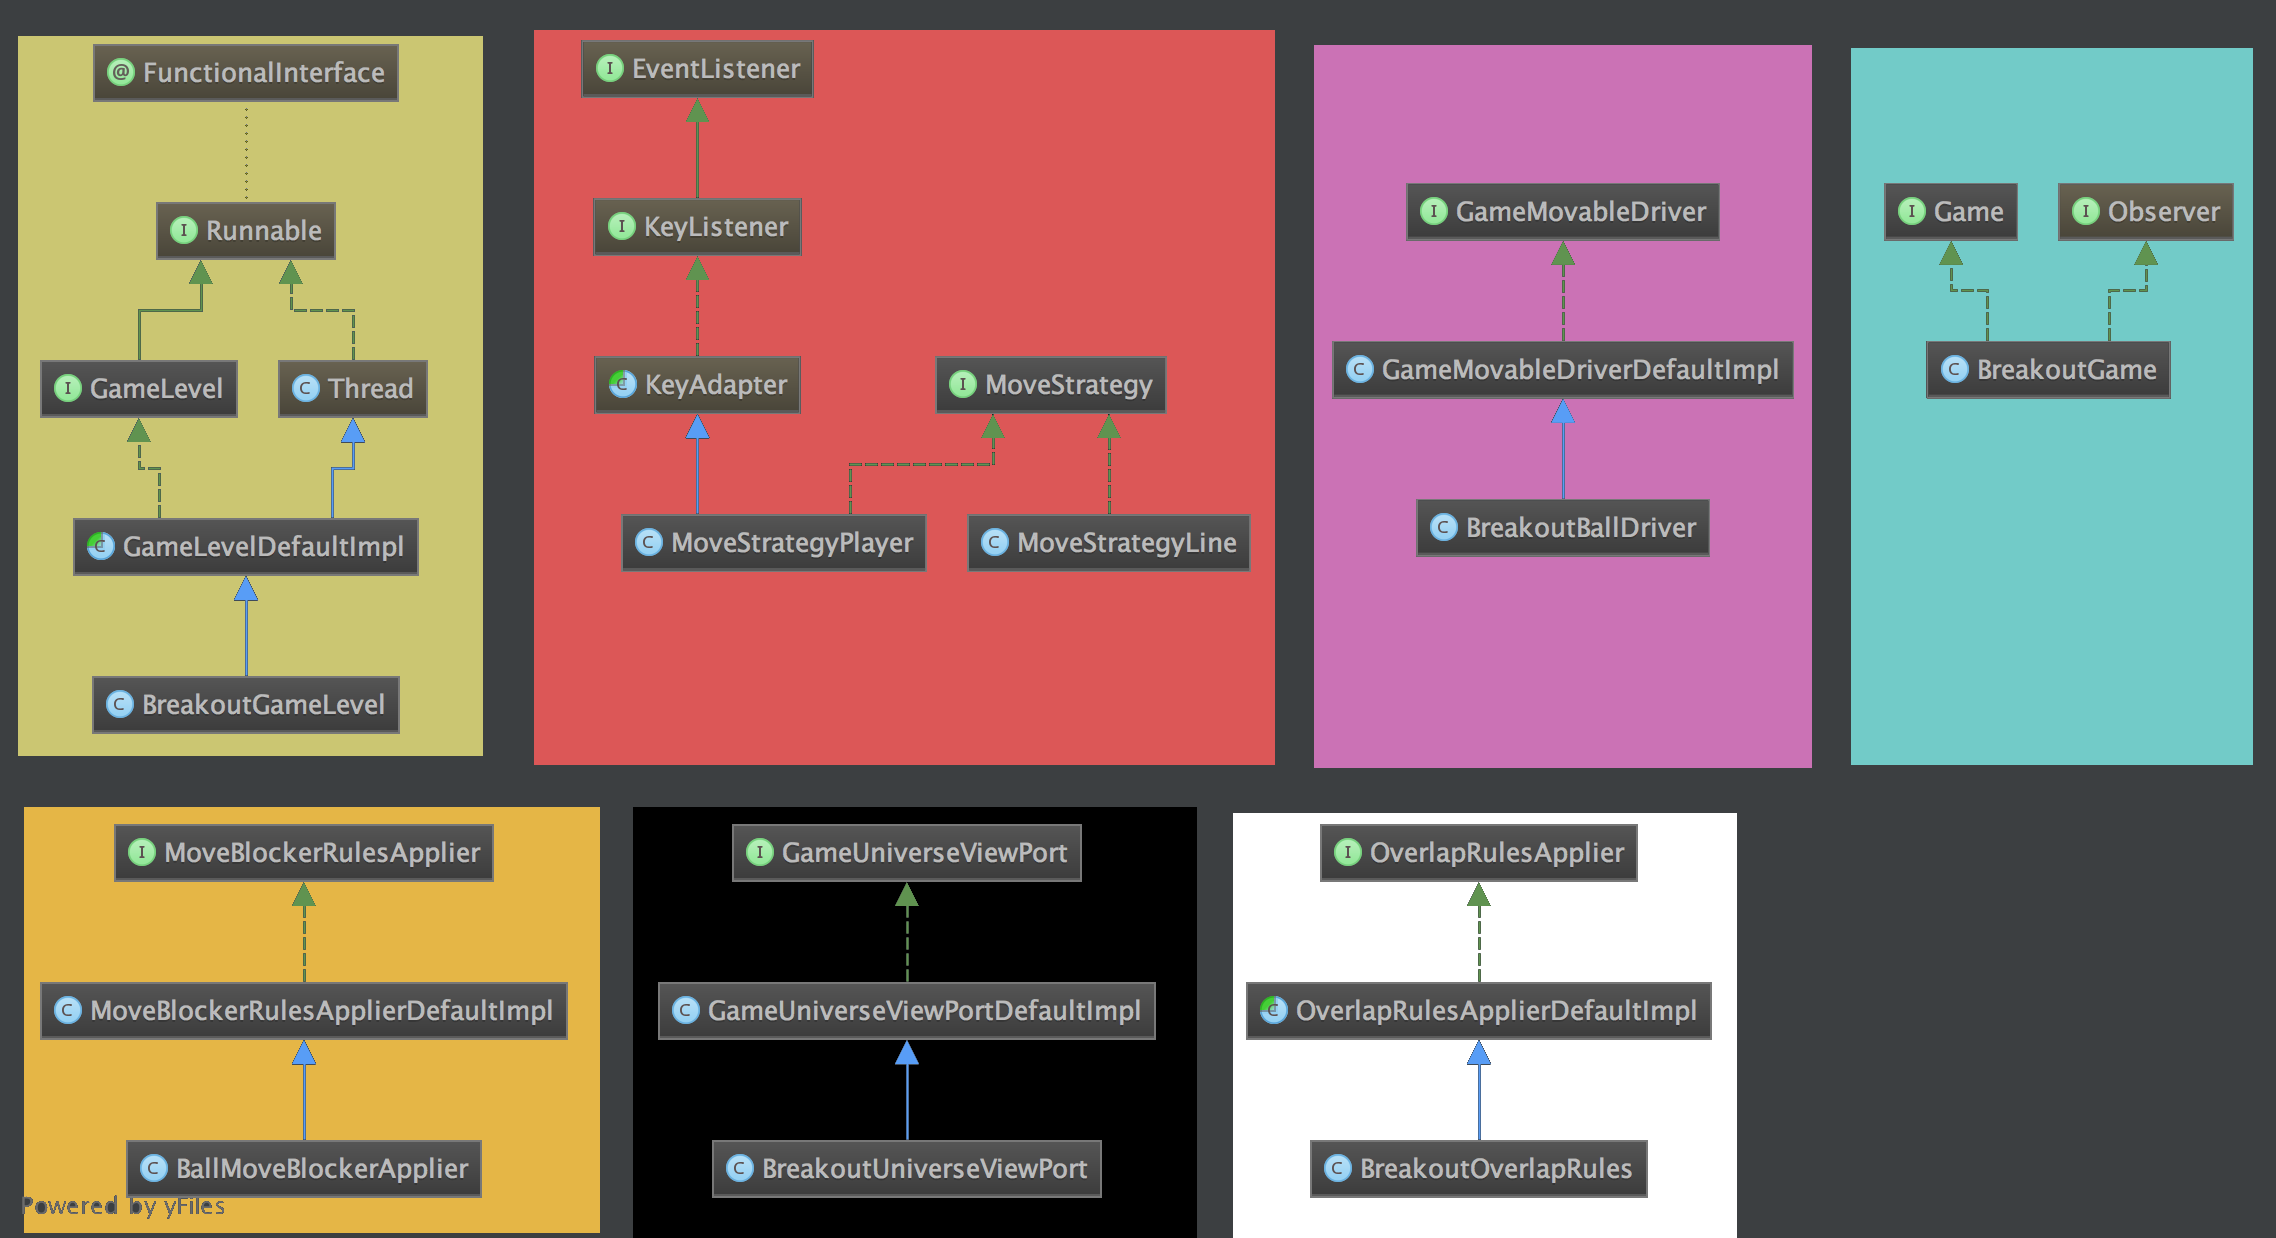
\includegraphics[scale=0.2]{images/severalDiagrams.png}
          	\caption{Multi diagramme de classe}
    		\end{center}
		\end{figure}
		\FloatBarrier
		\paragraph{Description :}
		Plusieurs classes forment de petits diagrammes de classes. Nous les avons regroupés dans une seule est même image. Pour les différencier
		nous avons utilisé un code couleur. Ce code couleur est détaillé dans la liste suivante : \\
		\begin{itemize}
		\item Diagramme jaune :
		\item Diagramme rouge :
		\item Diagramme violet :
		\item Diagramme bleu :
		\item Diagramme orange :
		\item Diagramme noir :
		\item Diagramme blanc :
		\end{itemize}
		
		
	
\subsection{Limites du jeu}
Cette partie sera utilisée pour expliquer quelles sont les limites du jeu. C'est à dire que nous expliquerons ce qui fonctionne mal ou ne fonctionne pas du tout.
\begin{itemize}
\item
\item
\item
\end{itemize}

\subsection{Difficultés rencontrées}
Nous avons tout de même rencontrées plusieurs difficultés et nous en ferons la liste dans cette partie. Nous donnerons également "l'état" de cette difficulté dans la version actuelle du jeu.
\begin{itemize}
\item
\item
\item
\end{itemize}


\section{Critiques du framework }
Nous consacrerons cette partie aux critiques que nous avons par rapport au framework fourni. Chaque critique sera accompagnée d'un cas dans lequel nous avons rencontré un problème suite aux limites du framework.
\begin{itemize}
\item
\item
\item
\end{itemize}

%\newpage
%\chapter{Conclusion}


\end{document}
\grid
